

\begin{figure}[h!]
\begin{center}
\centerline{\includegraphics[width=7cm]{../figures2/migration_diagram.eps}}
\caption{Migration diagram for focal player (defector on crossed site with $\text{payoff} = 1.3$). The best site in the migration range has highest payoff for the focal player (red-green site with $\text{payoff} = 1.3 \times 4 = 5.2$). The target site with highest payoff is occupied by a cooperative player and may be expelled with probability $s$ (orange arrow). In this case, the player on the target site is forced to move to the nearest empty site with $\text{payoff} = 2$ (black arrow pointing to light green site). However, with probability $1-s$, the focal player moves to the best empty site with $\text{payoff} = 2.6$ (blue arrow pointing to light green site).}
\label{fig:migration_diagram}
\end{center}
\end{figure}


\begin{figure}[h]
\begin{center}
\centerline{\includegraphics[width=16cm]{../figures2/phase_transition_d05.eps}}
\caption{{\bf a.} Phase transition of cooperation levels for migration Moore distances $M = \{1,3,5,7,11\}$ and population density $d=0.5$. For all migration ranges, a small level of property violation $s < 0.5\%$ enhances cooperation, while more property violation decreases cooperation. For $M=1$, cooperation decreases continuously as property violation grows (up to $s = 2\%$). For larger migration ranges, cooperation exhibits a linear decrease (given by $c \approx 1 - 2.2 \cdot s$) up to a critical phase transition point $s^*$. As $M$ increases, $s^{*}$ becomes a range of values (colored areas show the 1st to 99th percentile confidence intervals), where cooperation can either be sustained at high level ($c > 0.8$), or collapse as a result of a stochastic process: in this phase transition region, the outcome is independent of initial grid configuration. For instance, the critical phase transition range for $M=5$ (magenta area) is $3.7\% < s^{*} < 4.2\%$. While the outcome can either be high cooperation or collapse, the probability of high cooperation decreases within the critical phase transition range (cf.\ solid lines within areas): it becomes more likely that cooperation will collapse as property violation reaches the upper boundary of the critical range. {\bf b.} Phase transition areas as a function of population density: for each migration range represented by colored areas, the lower (dashed) boundary shows the limit below which cooperation thrives systematically ($c > 0.8$), while the upper (dash-dotted) boundary shows the limit beyond which cooperation collapses systematically. Larger migration ranges increase significantly the resistance to higher levels of property violation. However, the beneficial effects of long-range mobility are reduced for more densely populated worlds. Short-range mobility ($M=1$) is highly sensitive to property violation, regardless of population density.}
\label{fig:phase_transition}
\end{center}
\end{figure}


\begin{figure}[h]
\begin{center}
\centerline{\includegraphics[width=15cm]{../figures2/tseries_transition_3.eps}}
\caption{Evolution of expected payoff from player actions -- success-driven migration (green), property violation (blue), or strategy update (red). Expected payoff dynamics are initially very similar ($t< 10^5$ iterations) between thriving cooperation ({\bf a}) and collapse ({\bf b}) (same initial conditions: $d=0.5$, $M=5$, $s = 0.037$; colored areas show the 25\%--75\% percentile ranges). At $t \approx 10^5$ iterations, structural changes occur that determine the outcome: although cooperation continues to increase until $t \approx 5\times 10^5$, in the non-sustainable case ({\bf b}) strategy update (red) yields the highest expected payoff, while in the sustained cooperation case ({\bf a}), strategy update never provides the highest expected payoff. In the latter case, a subtle crossing occurs at the transition point $t \approx 10^5$, where migration transitions from the action with highest payoff to a lower payoff, while property violation becomes the action with highest expected payoff. Insets {\bf 1} and {\bf 2} show the correlograms between expected payoffs after the tipping point: in the sustainable case ({\bf a}), cross-dependence is very low, indicating strong decoupling between expected payoffs from different actions. In the collapsing scenario, cross-dependence remains high, with migration causing more property violation (green correlogram) and more strategy updates (red correlogram). In the unsustainable scenario, cooperation still increases long after the tipping point (until $t \approx 5\times10^{5}$) and then abruptly collapses. Panels {\bf c} and {\bf d} show expected mobility distance from success-driven migration (green), property violation (blue), and forced move (cyan). In the collapsing scenario ({\bf d}), expected mobility reaches a high plateau ($\log_{10} U_{\text{mobility}} \approx 2.5$), while for thriving societies ({\bf c}), expected mobility is lower ($1.5 < \log_{10} U_{\text{mobility}} < 2$), close to that of property violators ($\log_{10} U_{\text{expel}} \approx 1.5$). The dynamics presented for $d=0.5$ and $M=5$ are representative of phase transitions occurring for any game with $M>1$ and density $0.2 \leqslant d \leqslant 0.8$.}
\label{fig:tseries}
\end{center}
\end{figure}


\begin{figure}[h]
\begin{center}
\centerline{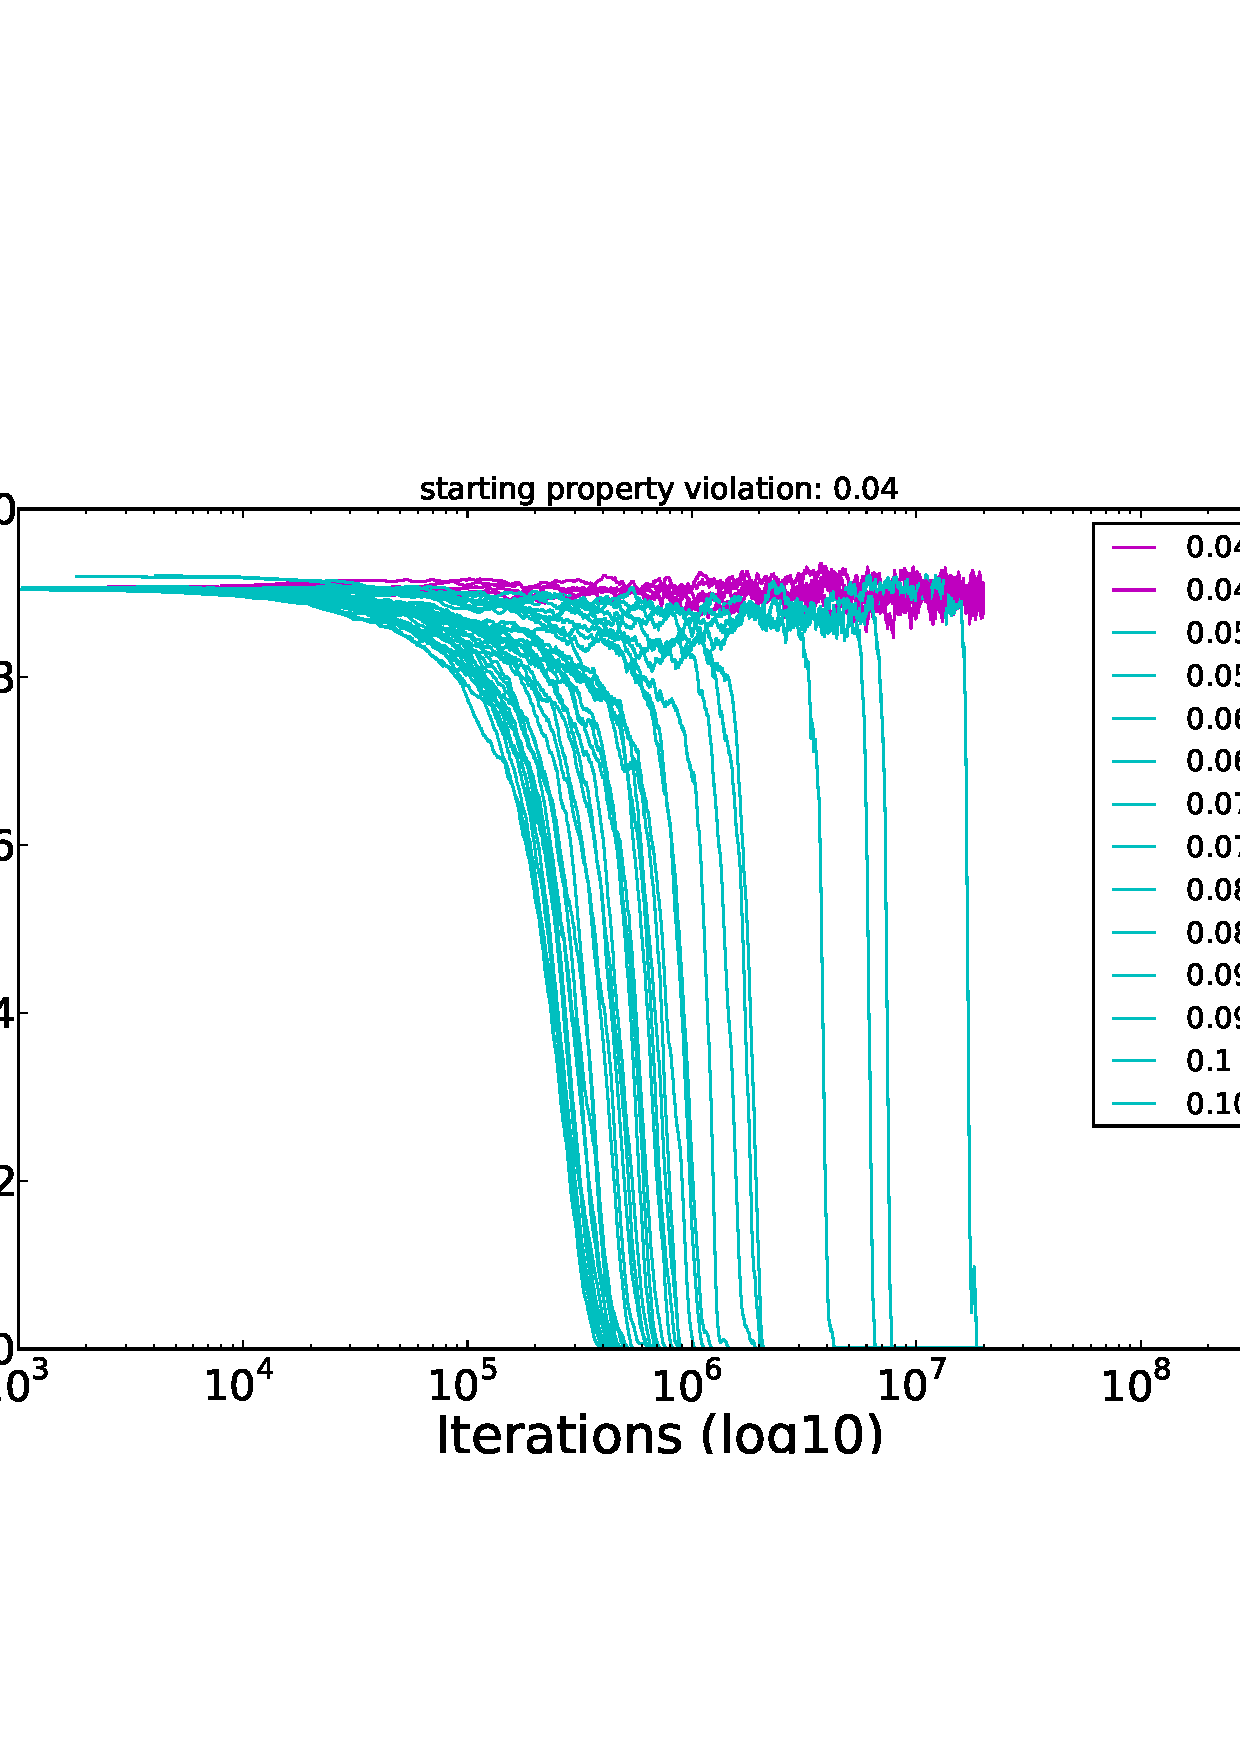
\includegraphics[width=11cm]{../figures2/resistance004.png}}
\caption{Evolution of cooperation when property violation is increased, starting from a simulation stabilized at high cooperation level ($c > 0.8$) and property violation in the upper range of the phase transition ($s=0.040$). For $s < 0.045$, cooperation remains high. For $0.05 \leqslant s \leqslant 0.06$, cooperation may collapse suddenly after $3\times10^6$ iterations, suggesting that any property violation value above the phase transition region may trigger collapse given enough time. For $s>0.06$, the cooperation curve decreases in a roughly parabolic shape that appears invariant in the limit of large $s$. The earliest that cooperation reaches zero is approximately $3 \times 10^5$ steps after the increase in property violation, indicating that even under large increases, a time window remains for corrective intervention.}
\label{fig:resistance}
\end{center}
\end{figure}

